%!TEX root = main.tex
\chapter{Design}
\label{chap:design}
In this chapter the design process will be explained in detail. We will show how our tool went from sketch to a fully working prototype. 
Through the different iterations of development, we made different design choices that helped design the application. Before the actual development began, we went
through a design process that resulted in a basis for implementation. In this section we will elaborate on how these steps culminated into the final design choice.
\section{Responsive web design}
Responsive web design\citep{responsivearticle} is a web design approach aimed at developing websites in order to provide an optimal viewing experience on a wide range of devices, from large desktop monitors to smartphones and tablets. This includes easy reading and navigation with minimal resizing, panning, and scrolling.

Any site designed to be responsive, adapts the layout to the viewing environment, along with fluid proportion-based grids and flexible images.

\begin{figure}[H]
\centering
	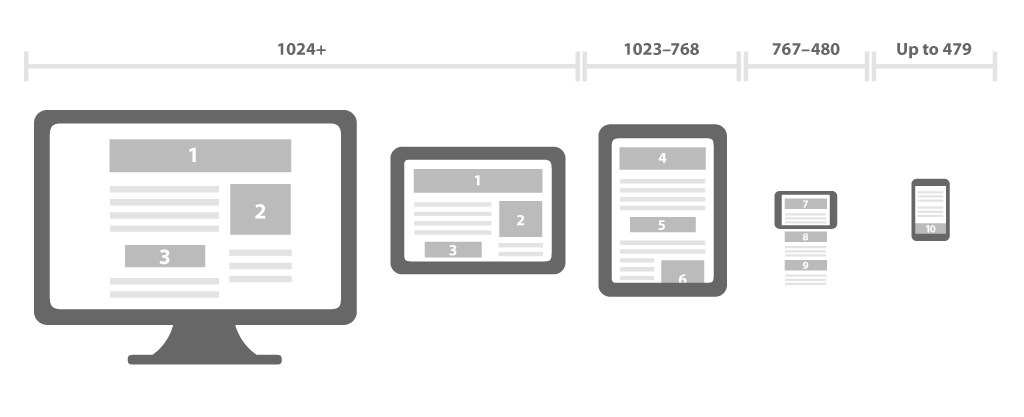
\includegraphics[width=\textwidth]{responsivelayout}
\caption{Responsive layout, adapting the same content to different viewing experiences \citep{responsivelayout}}
\label{responsivelayout}
\end{figure}

\subsection{Fluid grid}
A definition on fluid is : ``A fluid is a substance that continually deforms (flows) under an applied shear stress''\citep{fluidgrid}. In a web-design context, fluid will be the design and layout, and shear stress will be the device used to access the content.
Regardless of what the device or screen size is, components in fluid designs are going to flow and adapt to the user environment. Fluid grids define a maximum layout size and the grid is divided into columns for easier handling. These grids can then be designed with proportional widths and heights. The fluid grid and it's columns can be seen in Figure \ref{responsivelayout}.
The fluid grid\citep{fluidgrid, fluidarticle} concept states that page elements should be sized in relative units, like percentages or ems, instead of absolute units like pixels or points. Since fluid grids flow naturally based on the dimensions of its parent container-component, specific adjustments for various devices are therefore kept to a minimum. In the fluid grid, flexible images are also sized in relative units, up to 100\%, in order to prevent them from stretching outside their containing element\citep{fluidimages}. This means all kinds of elements on a web-page can be treated as proportions measured against their container, and not in absolute pixels. 

\section{Mockups}
At the very beginning we had an idea of what we wanted to do and how to do it. At the time we had not decided on a platform for our application. Because of this we sketched up some different design choices.

\subsection{Smartphone App}
Our first alternative was creating a native app for smartphones, on iOS or Android. We had experience with creating android applications before, so this was our first thought. 
\begin{figure}[H]
\centering
	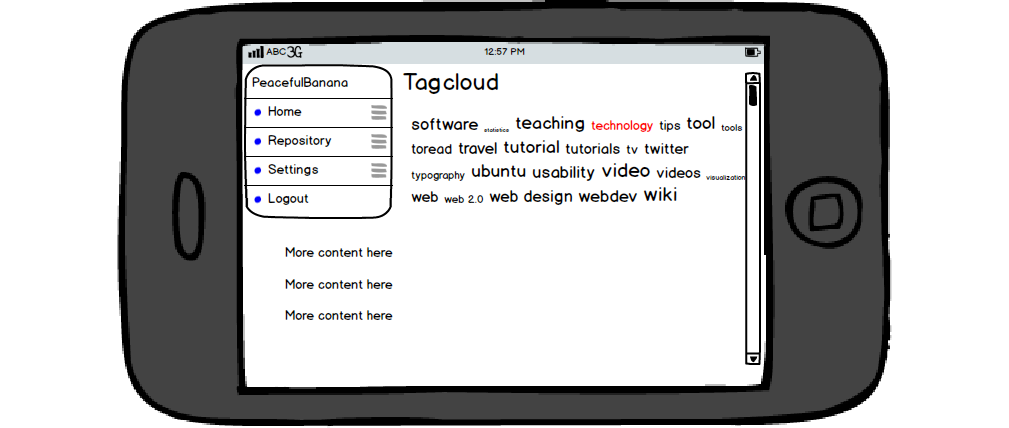
\includegraphics[width=\textwidth]{smartphonemock}
\caption{Smartphone mockup}
\label{smartphonemock}
\end{figure}

\subsection{Web-Application tool}
Our second option was creating our tool as a web-application. Web-applications are platform independent and can be accessed on a wide range of devices, as long as it has a fairly updated browser. The idea was to also make the web application responsive, which would provide an optimized viewing experience allowing for easy reading and navigation with minimal resizing, panning, and scrolling across a wide range of devices (from large monitors to mobile phones .\\
Figure \ref{webappmock} shows how our first sketch for a web-app looked like.
\begin{figure}[H]
\centering 
	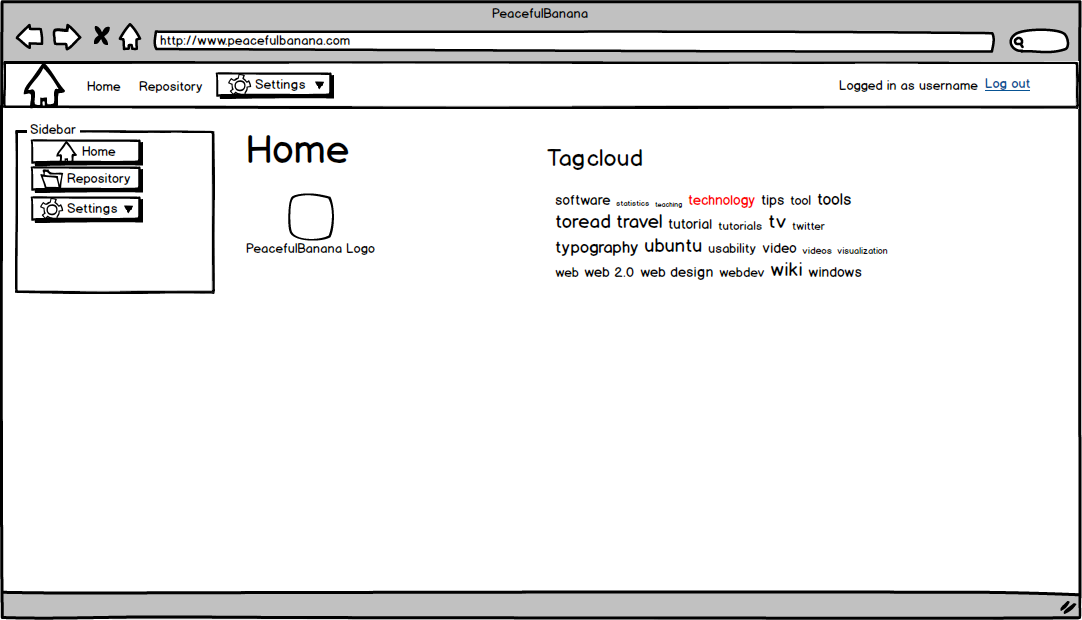
\includegraphics[width=\textwidth]{webappmock}
\caption{Web-app mockup}
\label{webappmock}
\end{figure}
As this was the main design options, we did some research on existing frameworks which might suit our requirements. The tool needed to be responsive and work on a wide range of devices, which made a fluid design suitable.

\section{Twitter Bootstrap}
The Twitter Bootstrap framework\citep{twitterbootstrap} features both the fluid grid and responsive web design requirements stated above. Bootstrap was developed by Mark Otto and Jacob Thornton at Twitter, as a framework to promote consistency in internal tools\citep{buildingbootstrap}. Twitter bootstrap is a free powerful front-end framework for faster and easier web development, and it's publicly available to use by anyone.

It contains HTML and CSS based design templates for interface elements like buttons, charts, and navigation. Bootstrap was made to not only look and behave optimally in desktop browsers, but in tablet and smartphone browsers via responsive CSS and HTML5 as well. The framework features responsive grids, components like tabs and dropdowns, JavaScript plugins, typography options and forms. 

Twitter Bootstrap is the most popular project in GitHub and is used by amongst others NASA(National Aeronautics and Space Administration)\citep{nasa}
Bootstrap is also modular, which means it is composed of a series of components that together make the toolkit. Developers can then cherry pick the components they need from the Bootstrap toolkit. 


\subsection{Bootstrap grid}
Bootstrap ships with the standard 940 pixel wide, grid layout. Developers can choose to use a variable-width layout if they wish. In any case the Bootstrap toolkit has four major variations in order to adapt content and grid width to different resolutions and devices: mobile phones, both portrait and landscape format, tablets and desktop computers with both low and high resolution and wide-screen support.

\subsection{Bootstrap components}
Bootstrap features a set of CSS style sheet, which defines styles for the major HTML elements. These style sheets allow for a platform-independent, multi browser enabled and consistent appearance for text, tables and other elements. \\
Bootstrap also comes with additional commonly used interface components. Such components are buttons, button-groups, buttons with drop-down option, navigation lists, tabs, breadcrumbs, pagination, different alerts and so on. 
\begin{figure}[H]
\centering
	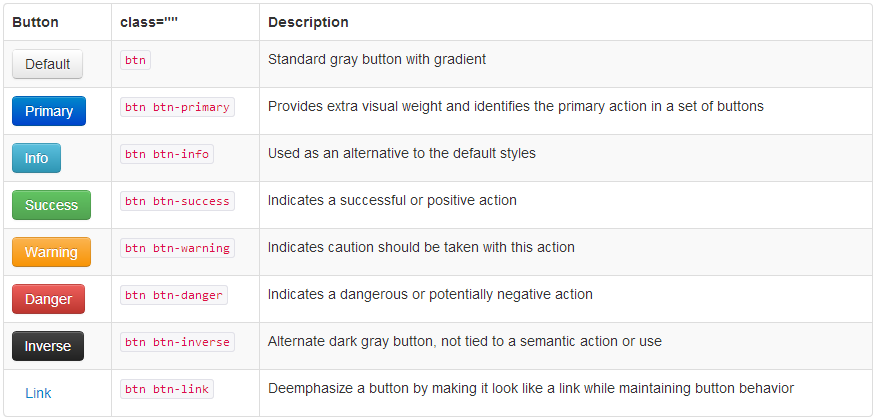
\includegraphics[width=\textwidth]{bootstrapbuttons}
\caption{Example of Twitter Bootstrap button types \citep{twitterbootstrap}}
\label{bootstrapbutton}
\end{figure}

\subsection{Icons}
Twitter Bootstrap comes with 140 sprite form icons, in both dark gray and white\footnote{Bootstrap icons: \url{http://twitter.github.com/bootstrap/base-css.html\#icons}} 

At their site they feature some examples that can be used as a basis for development. We decided to base our web application design on this layout, as it suited our needs and was very close to our initial mock-up
\begin{figure}[H]
\centering
	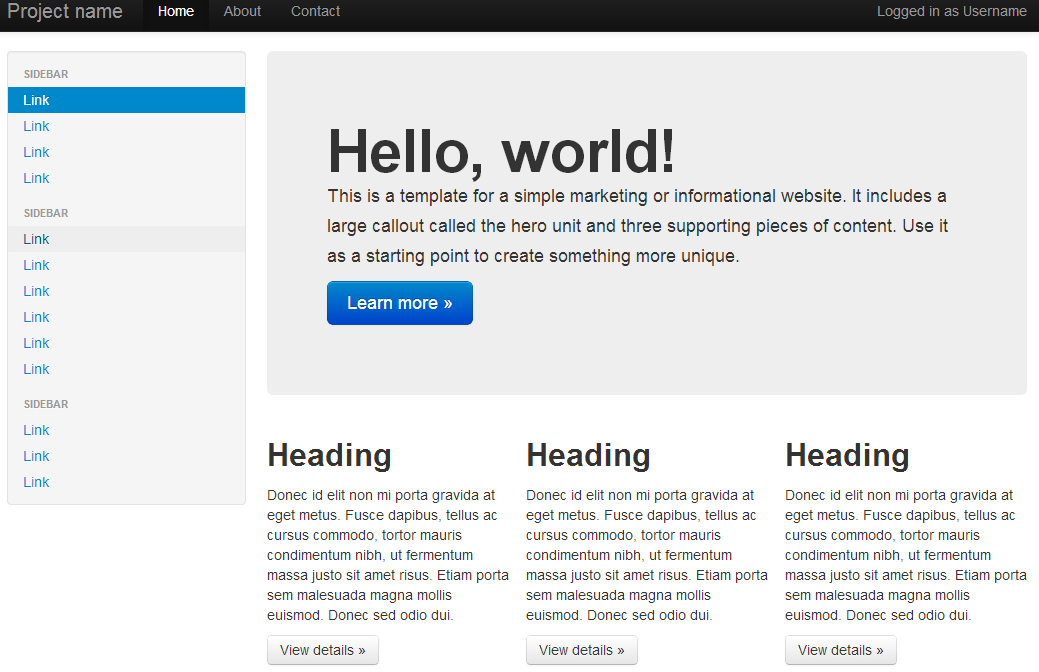
\includegraphics[width=\textwidth]{bootstrapexample}
\caption{Twitter bootstrap fluid layout with header and sidebar \citep{twitterbootstrap}}
\label{bootstrapexample}
\end{figure}

Visiting the site on a mobile device with a smaller screen, the responsive fluid layout would optimize the page to look like this:
\begin{figure}[H]
\centering
	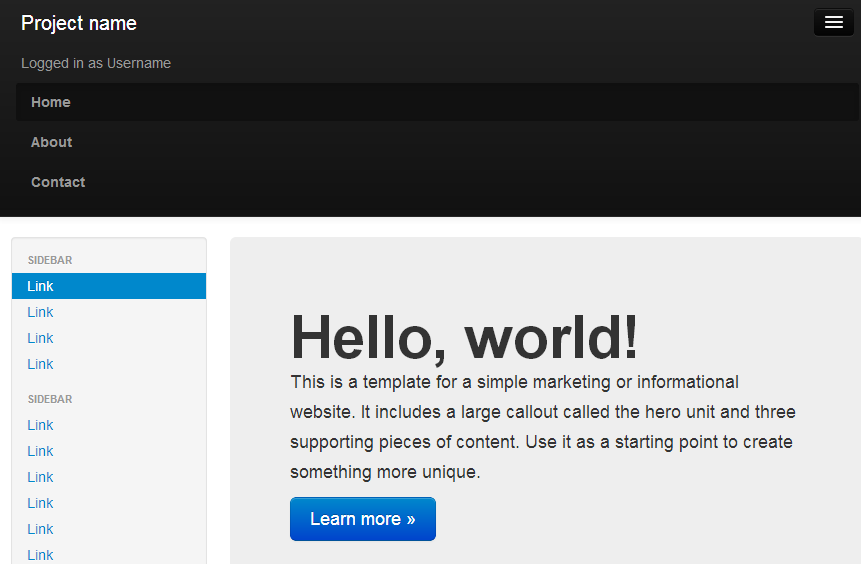
\includegraphics[width=\textwidth]{responsivemenuexample}
\caption{Twitter Bootstrap fluid layout with responsive menu and content \citep{twitterbootstrap}}
\label{bootstrapresponsive}
\end{figure}

And this is how our web-app looked after implementing bootstrap for a fully fluid and responsive web-application:
\begin{figure}[H]
\centering
	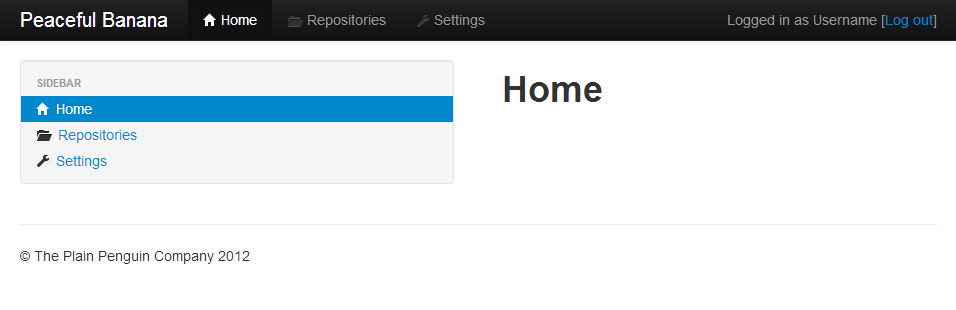
\includegraphics[width=\textwidth]{initial}
\caption{PeacefulBanana - Initial setup with Twitter Bootstrap}
\label{teamscreen}
\end{figure}

\section{PeacefulBanana Design}
After setting up and integrating the twitter bootstrap framework, the PeacefulBanana web-application was born, fully responsive and available on multiple platforms. This is how the final PeacefulBanana design looks like, it is based on the bootstrap example previously shown:
\begin{figure}[H]
\centering
	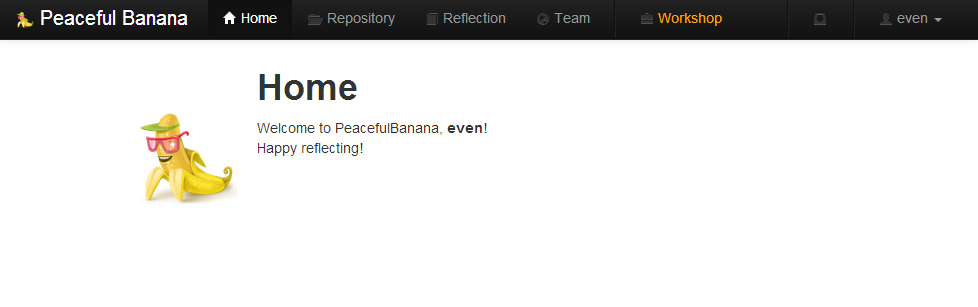
\includegraphics[width=\textwidth]{finalhome}
\caption{PeacefulBanana - Final home screen}
\label{finalhome}
\end{figure}
The design is based on the Twitter Bootstrap framework and the principles of responsive web-design and a fluid layout. More specifically it is based on the fluid layout example\footnote{\url{http://twitter.github.com/bootstrap/examples/fluid.html}}. The PeacefulBanana layout features a navigation-menu on top with different tabs, leading to different content. Each of these tabs contain sidebars, which acts as sub-menus. The tool also integrates a user-menu, which is a dropdown with different actions that relates to the user, like settings. 

\subsection{Icons}
The PeacefulBanana tool makes extensive use of the icons included in Twitter Bootstrap, in order to further define what action you can expect from a tab. For example a home icon on the \textit{Home} tab, a globe on the \textit{Team} tab and a user icon on the \textit{User dropdown}.
\begin{figure}[H]
\centering
	
\includegraphics[width=\textwidth]{iconexample}
\caption{Example of Twitter Bootstrap/Glyphicons use in PeacefulBanana \citep{twitterbootstrap}}
\label{iconexample}
\end{figure}

\subsection{MIRROR CSRL}
\label{subsec:mirrorcsrl}
This section describes the rationale behind the most important functionality implemented to PeacefulBanana, with relation to the Mirror CSRL cycle model. The section ends with a more detailed rationale behind the core functionality implemented. As described in Section \ref{mirrorsection} , the MIRROR CSRL model has four stages: 
\begin{enumerate}
    \item Plan and do work
    \item Initiate Reflection
    \item Conduct Reflection session
    \item Apply Outcome
\end{enumerate}
In this thesis, our research mostly focuses on the first two stages of the model, since PeacefulBanana is primarily to be used during work and as preparation for retrospective sessions. PeacefulBanana additionally includes some implementations focused towards the third stage \emph{Conduct reflection session}, as it also can be used during the session. 

\subsection{Plan and do work}
Figure \ref{plananddoworktable} shows functionality we implemented towards the \emph{Plan and do work} stage, and how our application help user(s) plan and perform their daily work tasks. 
Functionality in this stage is connected to \textbf{Sub research question 1}, which is focused on answering how the data collected from GitHub can be scaffolded in order to promote reflection. By carefully examining what GitHub offers itself, we could identify what they didn't offer and implement this functionality provided it could have a positive effect for promoting reflection for users. The challenge was not only to identify what data to collect, but also scaffold the collected data and present them to the users in a way that triggers reflection. 

Adding mood to the \emph{Daily Reflection Note} implementation gave us the opportunity to create a mood-graph based on the team user's mood every day. This representation allows for a quick and easy mood comparison, which may encourage user's to look into why their mood differs opposed to the team's in a certain period of time. Such a discussion might occur at any time, either because a user browses on his own and wants to discuss his findings, or the team browses it together.  
The rationale of adding notifications to the application was made in order to give users context-relevant feedback and remind them of the daily reflection notes. 

This functionality is also connected to \textbf{Sub research question 2}, which focuses on how to improve the tendency to reflect, both individually and in teams. 
\begin{figure}[H]
\centering
    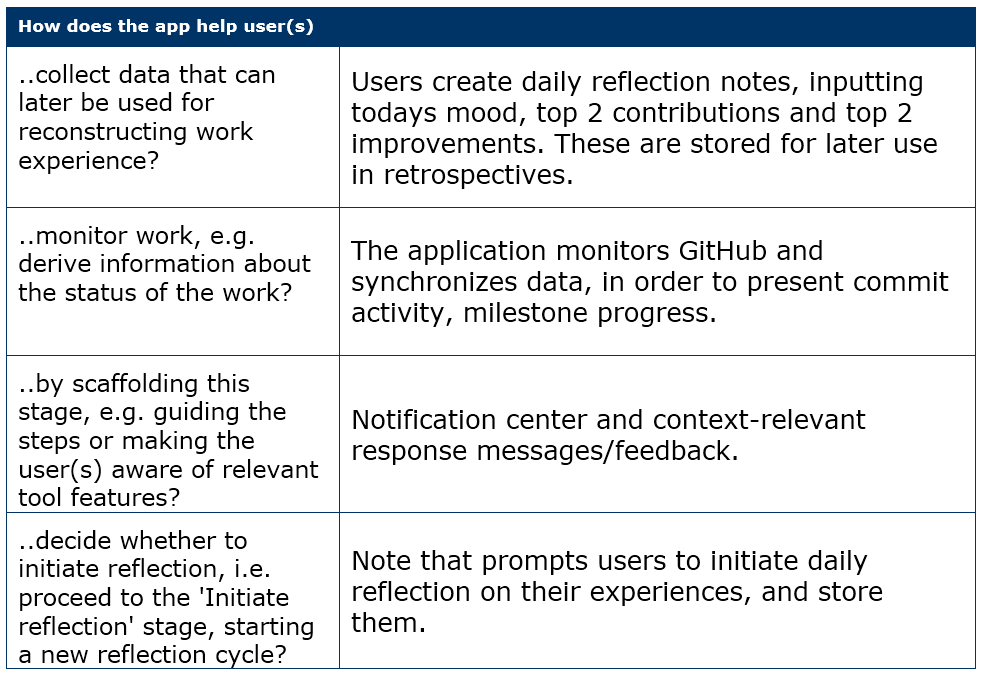
\includegraphics[width=\textwidth]{plananddoworktable}
\caption{Mirror CSRL Cycle - Plan and do work functionality \& implementations}
\label{plananddoworktable}
\end{figure}

\subsection{Initiate Reflection}
Figure \ref{initiatereflectiontable} shows functionality we implemented towards the \emph{Initiate Reflection} stage, and how our application help user(s) initiate reflection. Functionality in this stage is also coupled with \textbf{Sub research question 2}. The \emph{Reflection Workshop} functionality is implemented in order for teams to create a frame for their retrospective session. When a workshop has been added, individuals can also prepare by themselves by comparing their own data with the teams, i.e. the personal tag-cloud vs team tag-cloud and the mood-graph.  
\begin{figure}[H]
\centering
    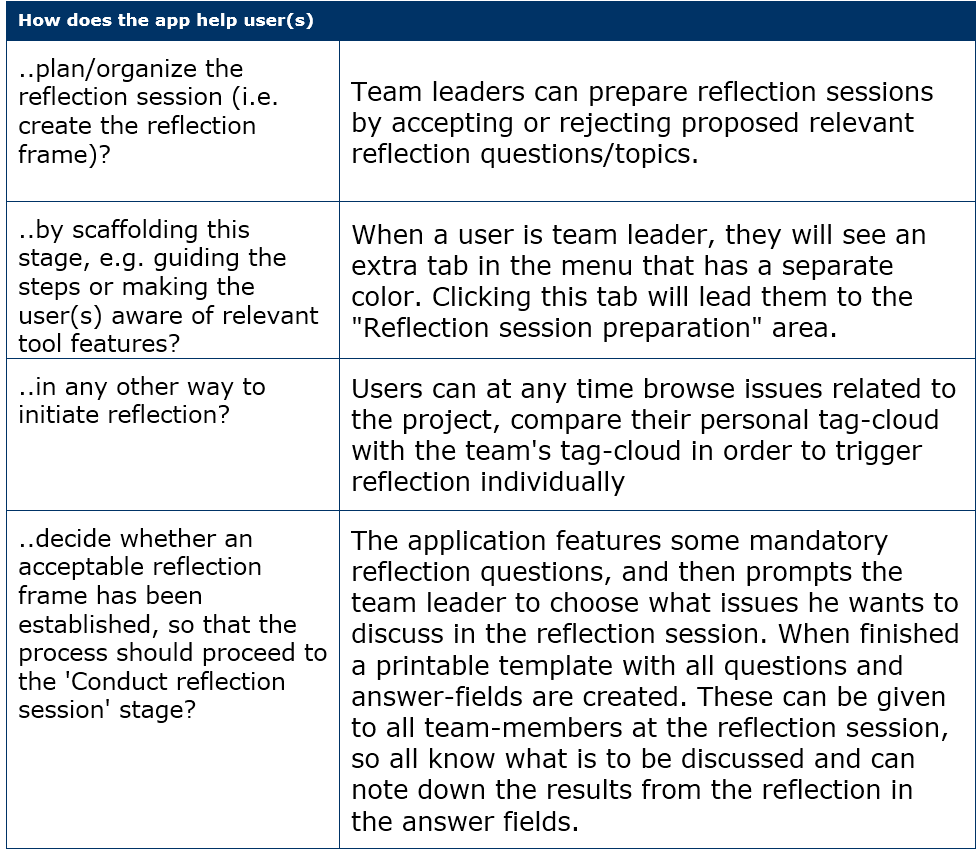
\includegraphics[width=\textwidth]{initiatereflectiontable}
\caption{Mirror CSRL Cycle - Initiate Reflection functionality \& implementations}
\label{initiatereflectiontable}
\end{figure}

\subsection{Conduct Reflection Session}
Figure \ref{conductreflectiontable} shows the functionality we implemented towards the \emph{Conduct Reflection Session} stage, and how our application help user(s) perform their retrospectives. 

This stage is not something we focused on, since most of the use of PeacefulBanana is doing daily work and using those data to prepare for retrospectives. Still the most notable functionality that is connected to this stage, is the ability to share and inspect reflection notes, meaning that teams can during reflection sessions wish to compare shared notes and create a discussion around these. Similarly teams can inspect repository data, like milestones and issues, and also tag-clouds connected to these. These tag-clouds can identify active issues which the team wishes to discuss during the retrospective. 
\begin{figure}[H]
\centering
    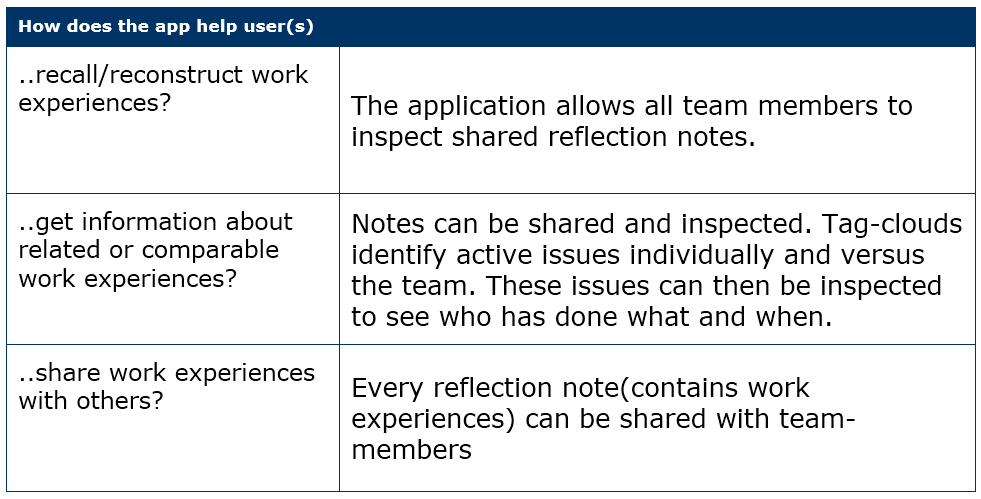
\includegraphics[width=\textwidth]{conductreflectiontable}
\caption{Mirror CSRL Cycle - Conduct reflection session functionality \& implementations}
\label{conductreflectiontable}
\end{figure}

\subsection{Core Functionality}
This section will describe the core functionality in the PeacefulBanana application and the relationship between the application and the CSRL model in section \ref{subsec:mirrorcsrl}. 
\paragraph{Daily reflection note}\mbox{}\\
Scaffolding is the act of creating a skeleton or a frame for the work to be done.
PeacefulBanana provides users with the ability to create reflection notes, where they reflect on that day's work and store it for later use. In this context the scaffolding is creating a frame for the reflection to be done, which includes text input and guiding questions. An example of such a reflection note can be seen in Figure \ref{dailynotefunc}. 

In order to encourage users to reflect on their daily work and to avoid generic or non-constructive input, we connected questions to each input field, to act as guidance. For each input, the application provides a question, like \emph{How did you feel about todays work?} for the mood input. Adding these questions helps users think back on their experiences that day and perform a reflection on these. 
\begin{figure}[H]
    \centering
        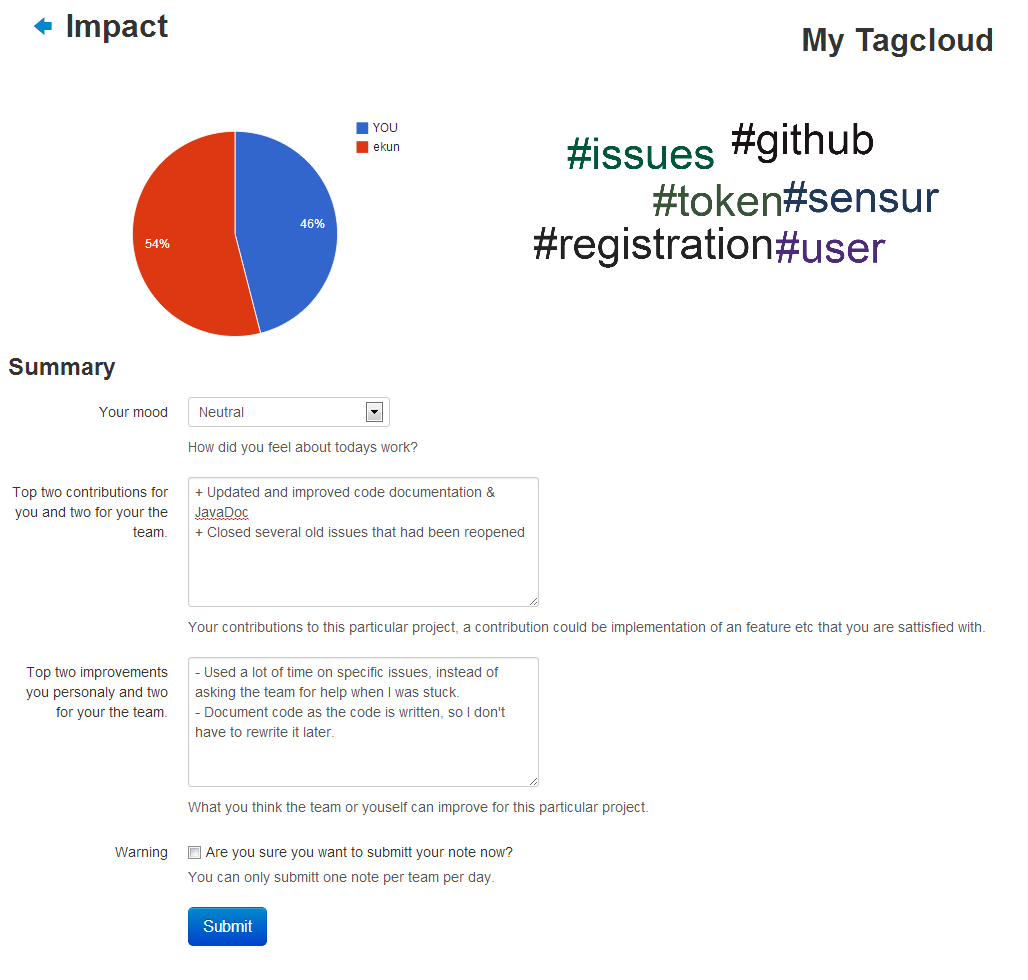
\includegraphics[width=\textwidth]{dailynote}
    \caption{PeacefulBanana reflection note}
    \label{dailynotefunc}
\end{figure}

\paragraph{Mood graphs}\mbox{}\\
When creating a reflection note, users can connect their current mood, that is how they felt, to the reflection note. By adding the ability to connect mood to notes each day, the tool can present meaningful mood-averages back to the users. These mood averages are used by PeacefulBanana to generate a mood-graph, depicting a user's or a team's mood over a period of time. 

By presenting this shared team-average mood, user's get an indication of how the work is perceived by the other group members and the team can create a discussion around certain trends in mood, or even why certain users stand out from the rest of the team's mood. 

An example of such a mood graph can be seen in Figure: \ref{moodgraphfunc}
\begin{figure}[H]
    \centering
        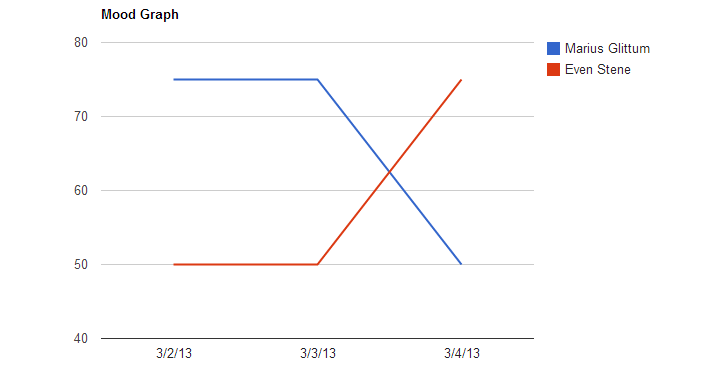
\includegraphics[width=\textwidth]{moodgraph}
    \caption{PeacefulBanana Team Mood-graph}
    \label{moodgraphfunc}
\end{figure}
\paragraph{Tag-clouds}\mbox{}\\
PeacefulBanana also provides the user with individual and team-wide tag-clouds. These tag-clouds are based on the user's or the team's activity in a GitHub project over a period of time. The tag-cloud elements are weighted according to how much the particular \emph{\#tag} has been worked with, the more activity the bigger the word. Implementation of the tag-clouds allows user's to see trending events in their own activity trajectory, but also compare it with the rest of the team. This enables the user to see how their work is affecting the team's work, but also gives the team an indication on what has been worked with over different periods of time(i.e. a development iteration). 
\begin{figure}[H]
    \centering
        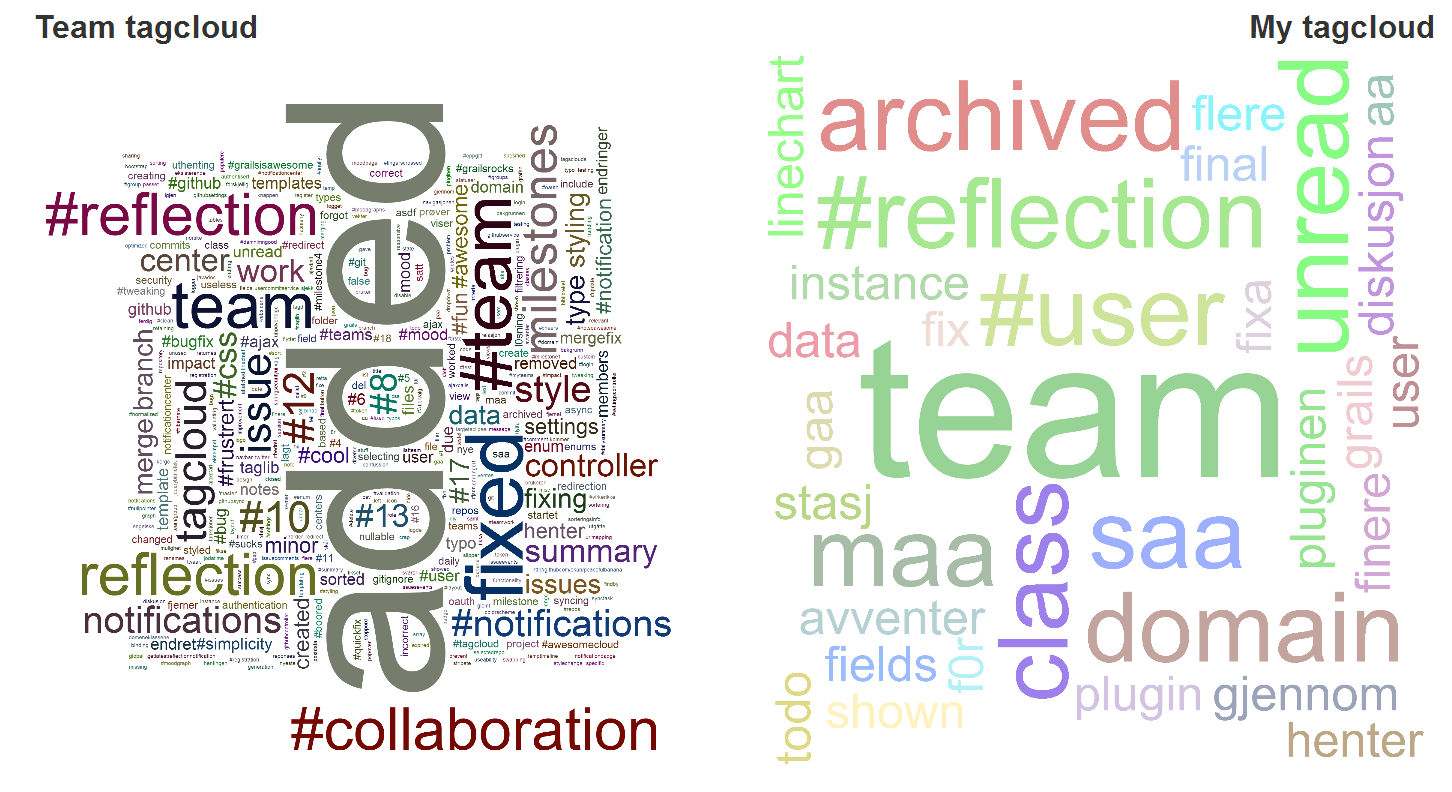
\includegraphics[width=\textwidth]{tagcloud_teamvsmy}
    \caption{PeacefulBanana tag-cloud implementation}
    \label{tagcloud_teamvsmy}
\end{figure}

\paragraph{Sharing of data}\mbox{}\\
Reflection notes can be shared with a user's team, should they want to.  PeacefulBanana collects team-relevant data from GitHub , scaffolds and presents these to users. This data gives the team the ability to see who is working on what, are there any trending issues in the team that can be intercepted and solved and more.  

Figure \ref{MyNotesFunc} shows how PeacefulBanana user's can see their notes and the notes' creation date, owning user, what team that user is on and the share status of the note. The user can also simply filter between their own notes or shared notes by their current team. This is shown in Figure \ref{notes_sharedfunc}
\begin{figure}[H]
    \centering
        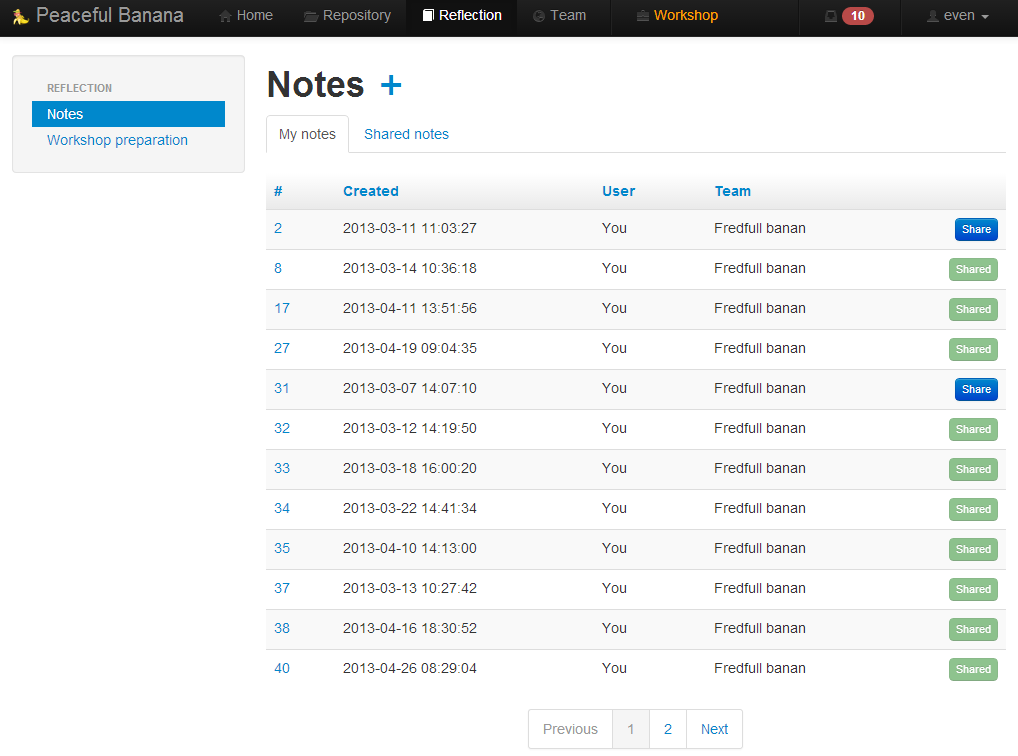
\includegraphics[width=\textwidth]{MyNotes}
    \caption{PeacefulBanana user notes}
    \label{MyNotesFunc}
\end{figure}
\begin{figure}[H]
    \centering
        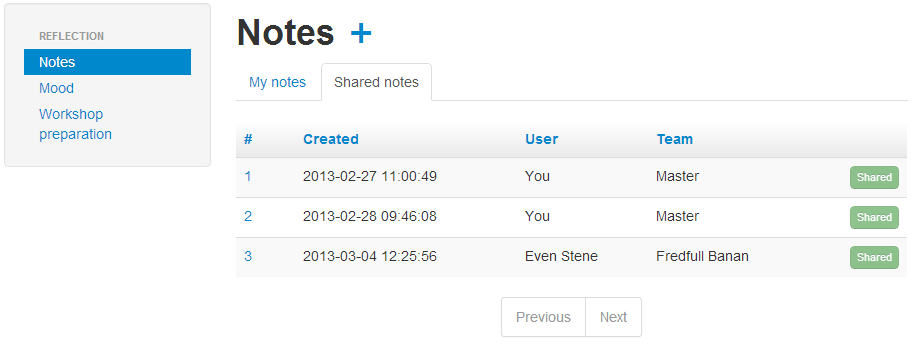
\includegraphics[width=\textwidth]{notes_shared}
    \caption{PeacefulBanana shared team notes}
    \label{notes_sharedfunc}
\end{figure}

\subsubsection{Repository}
In addition to functionality related to the \emph{Daily Reflection Note} and team retrospective sessions, we also implemented functionality aimed towards individual and collaborative reflection outside of these frames. This includes gaining an overview of the current project, the status of milestones and related issues. The rationale for implementing these functionalities is that we want to keep the required use of PeacefulBanana to a minimum, therefore only the 5-minute daily reflection is required to gain advantages towards the retrospective session. However, if a user or the whole team wants to dive deeper into the project data, they can do so in the \emph{Repository} section. Here users can see the teams commit activity, see the status of milestones and filter them based on this status. Clicking on a specific milestone will show all issues connected to the milestone and a tag-cloud containing that milestone's most used tags. Figure \ref{milestonefunc} shows an example of such a milestone with related issues, and Figure \ref{tagcloudfunc} shows the tag-cloud connected to this milestone. 

This means users or teams can identify certain issues that dominate, and can easily inspect these by clicking on them. Inspecting an issue will present comments, commit references and events concerning that issue. This enables individuals to inspect and revisit experiences, and allows teams to create a discussion around issues or milestones outside of the retrospective sessions. 

\begin{figure}[H]
    \centering
        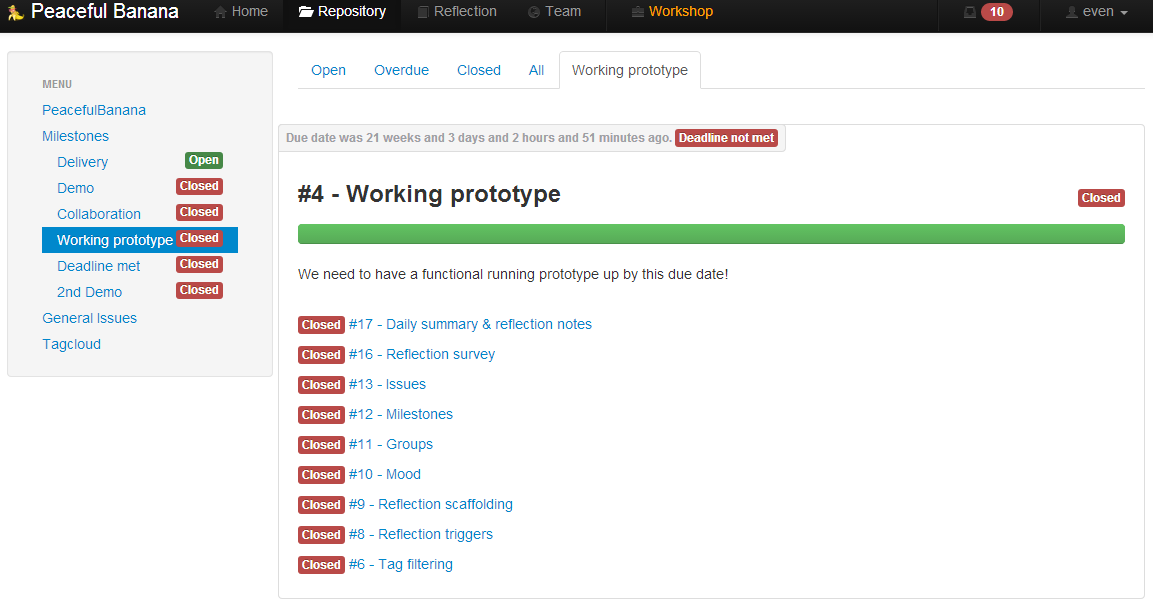
\includegraphics[width=\textwidth]{milestonefunc}
    \caption{PeacefulBanana - Repository milestone and issues}
    \label{milestonefunc}
\end{figure}

\begin{figure}[H]
    \centering
        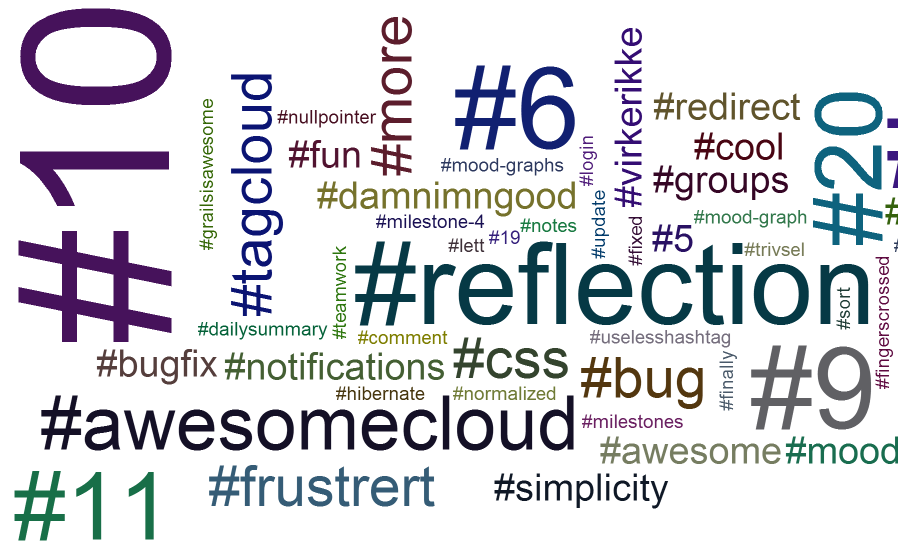
\includegraphics[width=\textwidth]{tagcloudfunc}
    \caption{PeacefulBanana - Repository milestone tag-cloud}
    \label{tagcloudfunc}
\end{figure}

\subsubsection{Reflection sessions}
One of the primary functionalities we implemented, in addition to the daily reflection note, was the \emph{Reflection Workshop}. The manager of each team will see a separate \emph{Workshop} tab. The workshop area allows managers to prepare for retrospective sessions, by creating a workshop for that period of time(i.e. an iteration that have lasted for the last two weeks). Figure \ref{workshopmandatoryfunc} shows an example of such a workshop. 

When the workshop has been created, users are met with three accordion headers\footnote{An accordion is a collapsible content panel for presenting information in a limited amount of space}. The accordions contain some mandatory questions which is some general reflection questions that is relevant to discuss in retrospective sessions, and so these cannot be removed from the workshop. The PeacefulBanana application also uses gathered data about the most used tags, to generate some proposed questions. The rationale behind this choice is that if the team has had a high activity with a certain tag, it is a high possibility that it's also important to discuss. Examples of these generated questions can be seen in Figure \ref{workshopgeneratedfunc}. Ultimately though, it is the manager of the team that chooses what questions or tags that should be discussed in the retrospective session. Therefore if the manager feels that one or more of the generated questions are unimportant, they can be removed. 

Finally the manager can browse a list of all tags, with the most active at the top, and simply click the tag that should be discussed as part of the retrospective session. If a tag is clicked under the \emph{Possible tags questions} they will be instantly moved to the \emph{Questions generated} section, and vice-versa deleted questions will be moved to the list of possible tag questions. Figure \ref{workshoppossiblefunc} shows how the tag list is presented in the application. 

\begin{figure}[H]
    \centering
        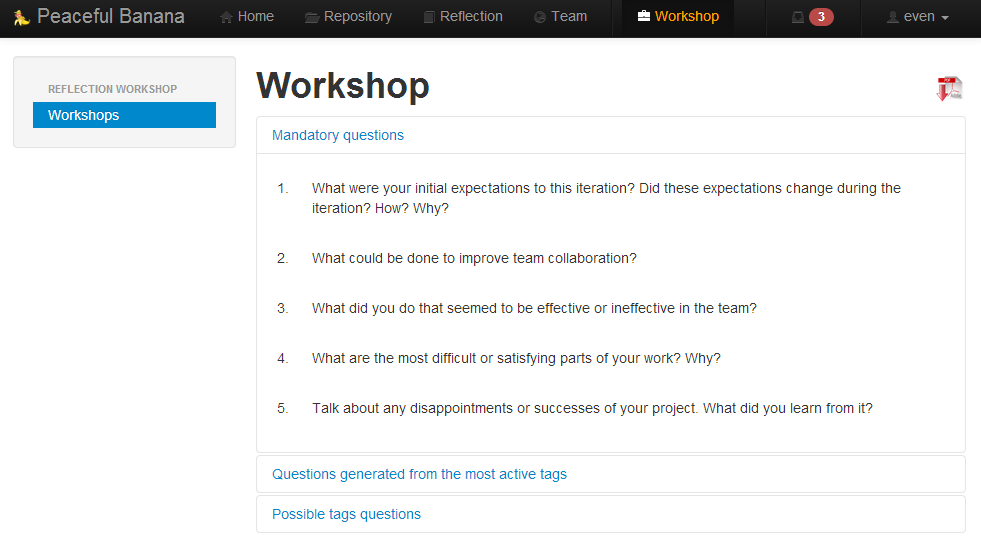
\includegraphics[width=\textwidth]{workshopmandatory}
    \caption{PeacefulBanana Workshop - Mandatory questions}
    \label{workshopmandatoryfunc}
\end{figure}
\begin{figure}[H]
    \centering
        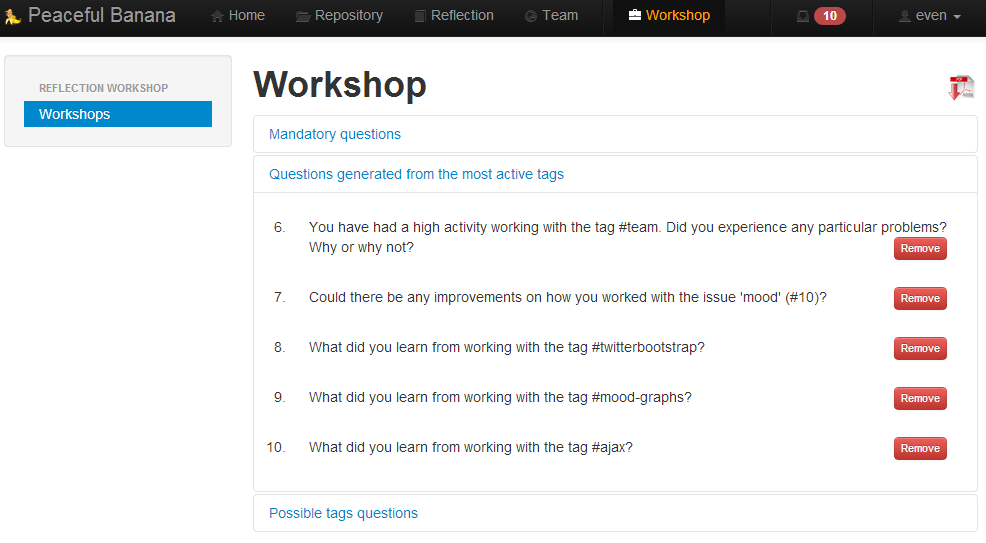
\includegraphics[width=\textwidth]{workshopgenerated}
    \caption{PeacefulBanana Workshop - Generated questions based on active tags}
    \label{workshopgeneratedfunc}
\end{figure}
\begin{figure}[H]
    \centering
        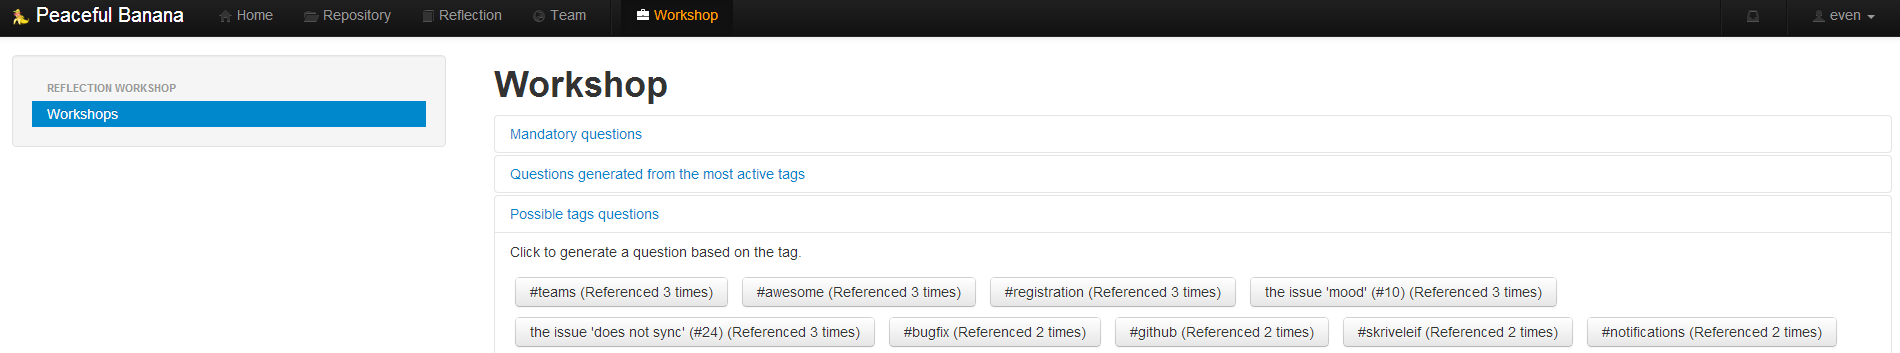
\includegraphics[width=\textwidth]{workshoppossible}
    \caption{PeacefulBanana Workshop - Possible questions based on tags}
    \label{workshoppossiblefunc}
\end{figure}

